\documentclass{article}
\usepackage{mathtools}
\usepackage{pgfplots}
\usepackage{amsmath}

\title{Pricing and Inventory Control For High Frequency Market Making}
\author{Dar En Tang}
\begin{document}
\maketitle
\section{Pricing}
The inventory at time $t$ is denoted as $q(t)$.
A discount $\delta$ is applied to the bid and ask prices for inventory control. It is defined by the polynomial:
\begin{equation}
    \delta = - \text{sign}(q(t)) \lfloor a|q(t)|^n \rfloor
\end{equation}

Where $a$ and $n$ determines the ``harshness'' of the penalty. For example, these two parameters can be defined
by specifying the inventory level at which one penalisation level is applied, $q_1$, and
the penalisation level at the maximum allowable inventory level, $\delta_\text{max}$ at $q_\text{max}$.
\begin{figure}[h]
    \centering
    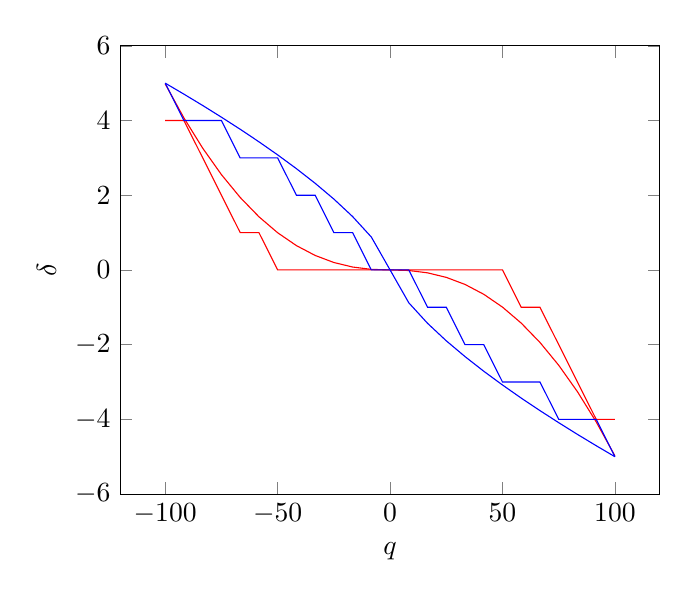
\begin{tikzpicture}
        \begin{axis}[ 
        xlabel=$q$,
        ylabel={$\delta$}
        ] 
        \addplot[red, domain=-100:100]{-sign(x) * floor(0.000113 *abs(x) ^ 2.322)}; 
        \addplot[red, domain=-100:100]{-sign(x) * (0.000113 *abs(x) ^ 2.322)}; 
        \addplot[blue, domain=-100:100] {-sign(x) * floor(0.2 * abs(x) ^ 0.699)}; 
        \addplot[blue, domain=-100:100] {-sign(x) * (0.2 * abs(x) ^ 0.699)}; 
        \end{axis}
    \end{tikzpicture}
    \caption{Penalty levels in response to inventory}
\end{figure}
For instance, if $q_1$ is 15 and $q_\text{max}$ and $\delta_\text{max}$ are 100 and 5 respectively, then
$n = 2.322, a = 0.000113$. If we wish to penalise heavier, then $q_1$ can be set to a stricter
value of 10, resulting in $n = 0.699, a = 0.2$. In general, setting a smaller $q_1$ will result in a smaller
fluctuation in inventory, and a higher $q_\text{max}$ will result in a quicker ``unstuck''. Although please note
that this is a trade off between stability and profitability, as any penalty applied to the price will result
in suboptimal ordering.\\
\\Now, let the best ask and best bid in the etf order book be $p^a_e$ and $p^b_e$ respectively. In 
the future order book, same convention applies, i.e. $p^a_f$ and $p^b_f$. The asking price is defined by:

\begin{equation} \label{eqn:ask}
p^a = \begin{cases} \max(p^a_e + \delta, p^a_f) & q < q_\text{thres} \\ \min(p^a_e, p^a_f) & \text{otherwise} \end{cases}
\end{equation}

Where $p_\text{thres}$ is the threshold inventory volume. In general, smaller $q_\text{thres}$ will result in a more stable inventory. 
This value can set to be dependent on the current movement in the market:
\begin{equation}
    q_\text{thres} = {\min(q_\text{thres}}_\text{max}, f|\dot{p_e}|)
\end{equation}

Where ${q_\text{thres}}_\text{max}$ is the maximum threshold value, and $f$ is some multiplier, typically
$f = 0.4$. In a similar fashion, the bidding price can be defined as:

\begin{equation} \label{eqn:bid}
p^b = \begin{cases} \max(p^b_e, p^b_f+\delta) & q < -q_\text{thres} \\ \min(p^b_e, p^b_f) & \text{otherwise} \end{cases}
\end{equation}

Now, equations \ref{eqn:ask} and \ref{eqn:bid} are discontinuous functions. To smooth the transition
between the two, a mixing multiplier $\lambda$ can be used, which can be defined from a logistic curve:

\begin{eqnarray}
    \lambda^a &= \dfrac{1}{1 + \exp{(-\kappa (q - q_\text{thres})})} \\ 
    \lambda^b &= \dfrac{1}{1 + \exp{(-\kappa ( - q - q_\text{thres}))}}
\end{eqnarray}

Where $\kappa$ is a mixing constant. A larger $\kappa$ results in a stepper transition in the sigmoid curve.

In turn, equations \ref{eqn:ask} and \ref{eqn:bid} can be redefined as:

\begin{eqnarray}
    p^a &= \lambda \max(p^a_e + \delta, p^a_f) + (1 - \lambda)\min(p^a_e, p^a_f)\\
    p^b &= \lambda \max(p^b_e, p^b_f + \delta) + (1 - \lambda)\min(p^b_e, p^b_f)
\end{eqnarray}


\end{document}